\lstset{language=Java}
\section{Suche}\label{search}
Baguette verwendet eine sequentielle, rekursive Suche auf Grundlage vom Min/Max-Algorithmus und Alpha/Beta Pruning, um beste Z\"uge mithilfe dem parallel generierten Suchbaum zu finden.
Die Suche wird wiederholt, bei erreichen neuer Tiefen im Suchbaum gestartet.
Es handelt sich dabei also um eine iterative Suche.

\subsection{Min/Max-Algorithmus}
Der Min/Max-Algorithmus ist ein grundlegendes Verfahren um einen besten Zug aus dem Suchbaum zu finden.
Der minimierende Spieler ist dazu bestrebt den Zug mit niedrigstem Wert zu w\"ahlen.
Der maximierende Spieler ist dazu bestrebt den Zug mit dem h\"ochsten Wert zu w\"ahlen.
Diese Werte werden dabei bis zur Wurzel getragen, bei welcher dann entsprechend der beste Zug f\"ur den jeweils am Zug befindlichen Spieler gew\"ahlt wird.
Durch dieses Prinzip w\"ahlt der am Zug befindliche Spieler also immer den Zug mit dem geringsten Schaden bzw den Zug mit dem gr\"ossten Vorteil.
Eine Vorbedingung f\"ur ein sinnvolles Ergebnis des Min/Max-Algorithmus ist, dass alle Blattknoten im Suchbaum auf der selben Tiefe liegen,
da h\"oher liegende Knoten sonst tiefer liegende Knoten verdecken w\"urden.
\\\\
Beispiel:\\Jeder Knoten stellt einen m\"oglichen Zug dar.
\begin{figure}[h]
\begin{center}
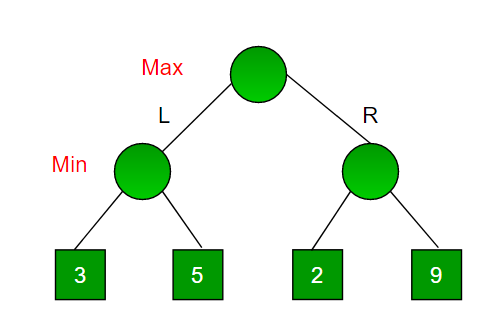
\includegraphics[scale=0.5]{minmax.png}
\caption{source: www.geeksforgeeks.org/minimax-algorithm-in-game-theory-set-1-introduction}
\end{center}
\end{figure}

Wir beginnen bei dem minimierenden Knoten links.
Dieser w\"ahlt das Minimum zwischen 3 und 5, also 3.
Dieser Knoten hat also nun den Wert 3.\\
Gehen wir nun zum minimierenden Knoten Rechts \"uber.
Dieser w\"ahlt das Minimum zwischen 2 und 9, also 2.
Dieser Knoten hat also nun den Wert 2.
Als letztes betrachten wir den maximierenden Knoten und somit gleichzeitig die Wurzel.
Dieser w\"ahlt das Maximum zwischen 3 und 2, also 3.
Der beste Zug der an der Wurzel gew\"ahlt werden kann ist also der rechte.

\section{Alpha/Beta Pruning}
Alpha/Beta Pruning ist eine Erweiterung des Min/Max-Algorithmus, durch die nicht alle Knoten im Suchbaum betrachtet werden m\"ussen.
Dadurch kann, bei gleichbleibendem Ergebnis, Zeit eingespart werden und somit tiefere Ebenen im Suchbaum erreicht werden.
\\\\
Prinzip anhand eines Beispiels.
Die Berechnung des besten Wertes f\"ur folgenden Suchbaum sieht wie folgt aus:
\begin{flushleft}
max\{ min\{3,5,10\}, min\{2,a,b\}, min\{2,7,3\}\}\\ = max\{3,c,2\}\\ = 3      $$a,b,c \in \mathbb{N}$$
\end{flushleft}
3 ist dabei das richtige Ergebnis, da unabh\"angig von a und b, $c<=2$ sein muss.
In Worten bedeutet das, dass der Zug mit den Unbekannten nicht weiter durchsucht werden muss, da er durch den Wert 2 bereits schlechter werden kann als der linke Zug mit wert 3.

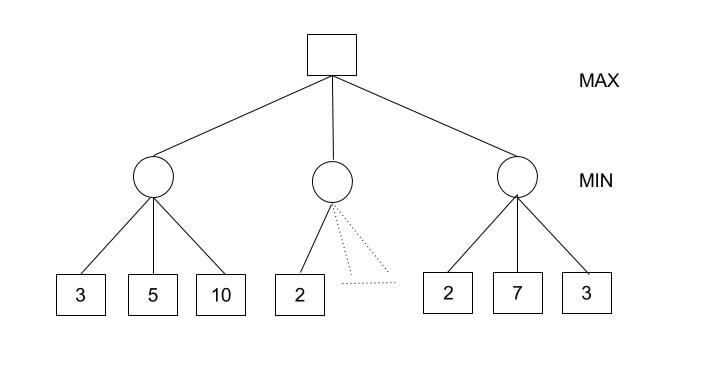
\includegraphics[scale=0.5]{alpha-beta-pruning.jpg}\\
\begin{tiny}
Beispiel und Bild entnommen von: hackerearth.com/blog/developers/minimax-algorithm-alpha-beta-pruning
\end{tiny}\\
Alpha und Beta sind die Namen der Variablen , die verwendet werden um zu \"uberpr\"ufen, ob der Wert eines Knotens bereits schlechter ist, als der eines vorher besuchten Knotens.
Alpha wird nur vom maximierenden Spieler ver\"andert und Beta nur vom minimierenden Spieler.
Wenn Alpha gr\"osser als Beta ist, kann die Suche auf dem aktuellen Knoten abgebrochen werden.
\\\\
Hierzu vereinfachter Code der Alpha/Beta Funktion wie sie in Baguette verwendet wird.
Da die Funktion selbst nur einen Wert zur\"uck gibt, wird in der letzten if Bedingung zus\"atzlich die globale BestMove Variable mit dem gefundenen besten Zug gesetzt, wenn der aktuell untersuchte Knoten die Wurzel des Suchbaum ist.
\newline
\begin{lstlisting}[frame=single]
int alphaBetaSearch(parent, maxDepth, alpha, beta) {
        bestValue = parent.blacksTurn() ?
                MAX_VALUE : MIN_VALUE;

        if (parent.getDepth() == maxDepth) {
            return parent.getValue();
        } else {
            for (int i = 0; i < children.length; i++) {
                curValue = alphaBetaSearch
                (children[i], maxDepth, alpha, beta);

                if (parent.blacksTurn()) {
                    if (curValue < bestValue) {
                        bestValue = curValue;
                        beta = curValue;
                        bestMove = children[i];
                    }
                } else {
                    if (curValue > bestValue) {
                        bestValue = curValue;
                        alpha = curValue;
                        bestMove = children[i];
                    }
                }
                if (beta <= alpha) {
                    break;
                }
            }
            if (parent == ROOT) {
                setBestMove(bestMove);
            }
         return bestValue;
\end{lstlisting}

